% CLP-CSGM Ridge cross-well Vc section fragment.
% Generated by scripts/csgm_m2_finalize_artifacts.py.

\section{Conditional CSGM for sparse core assimilation}
\label{sec:csgm_m2}

We evaluate a conditional compressed-sensing-with-generative-models (CSGM)
variant on the cross-well Vc low-data benchmark. The decoder $G(z)$ is trained
as an autoencoder prior over Vc windows, while a ridge model predicts a latent
prior $z_0=h(u)$ from the wireline logs. Sparse measurements enter through a
test-time inverse problem,
\[
  \hat z = \arg\min_z \|M G(z)-b\|_2^2
  + \lambda \|z-z_0(u)\|_2^2,
  \qquad \hat y = G(\hat z).
\]
This differs from direct \([u,b]\to y\) baselines because \(b\) is enforced as
a measurement-consistency constraint rather than treated only as an input
feature.

\begin{figure}[t]
  \centering
  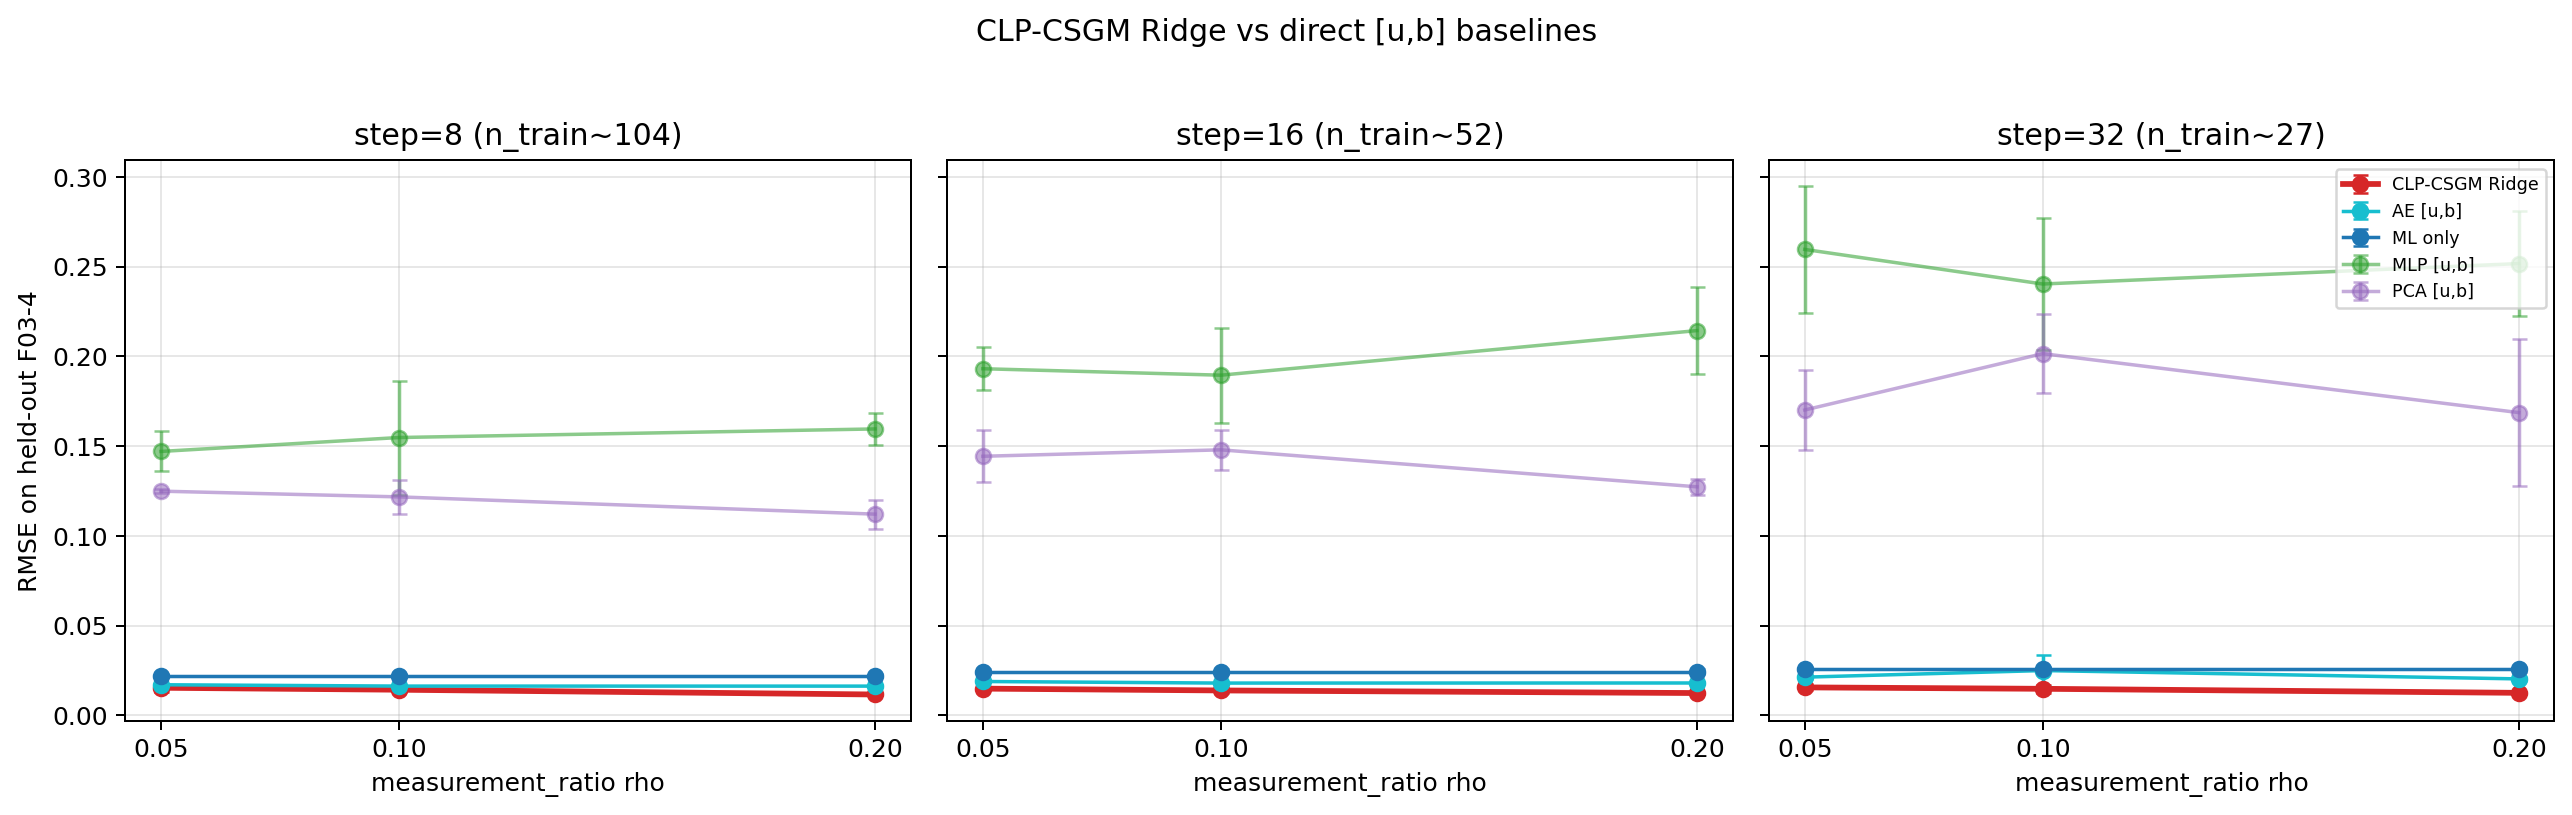
\includegraphics[width=\linewidth]{figures/csgm_m2_grid/01_rmse_vs_measurement_ratio.png}
  \caption{CLP-CSGM Ridge versus direct baselines on cross-well Vc low-data regimes.
  Each panel fixes the sliding-window step and varies the measurement ratio.}
  \label{fig:csgm_m2_rmse}
\end{figure}

\begin{figure}[t]
  \centering
  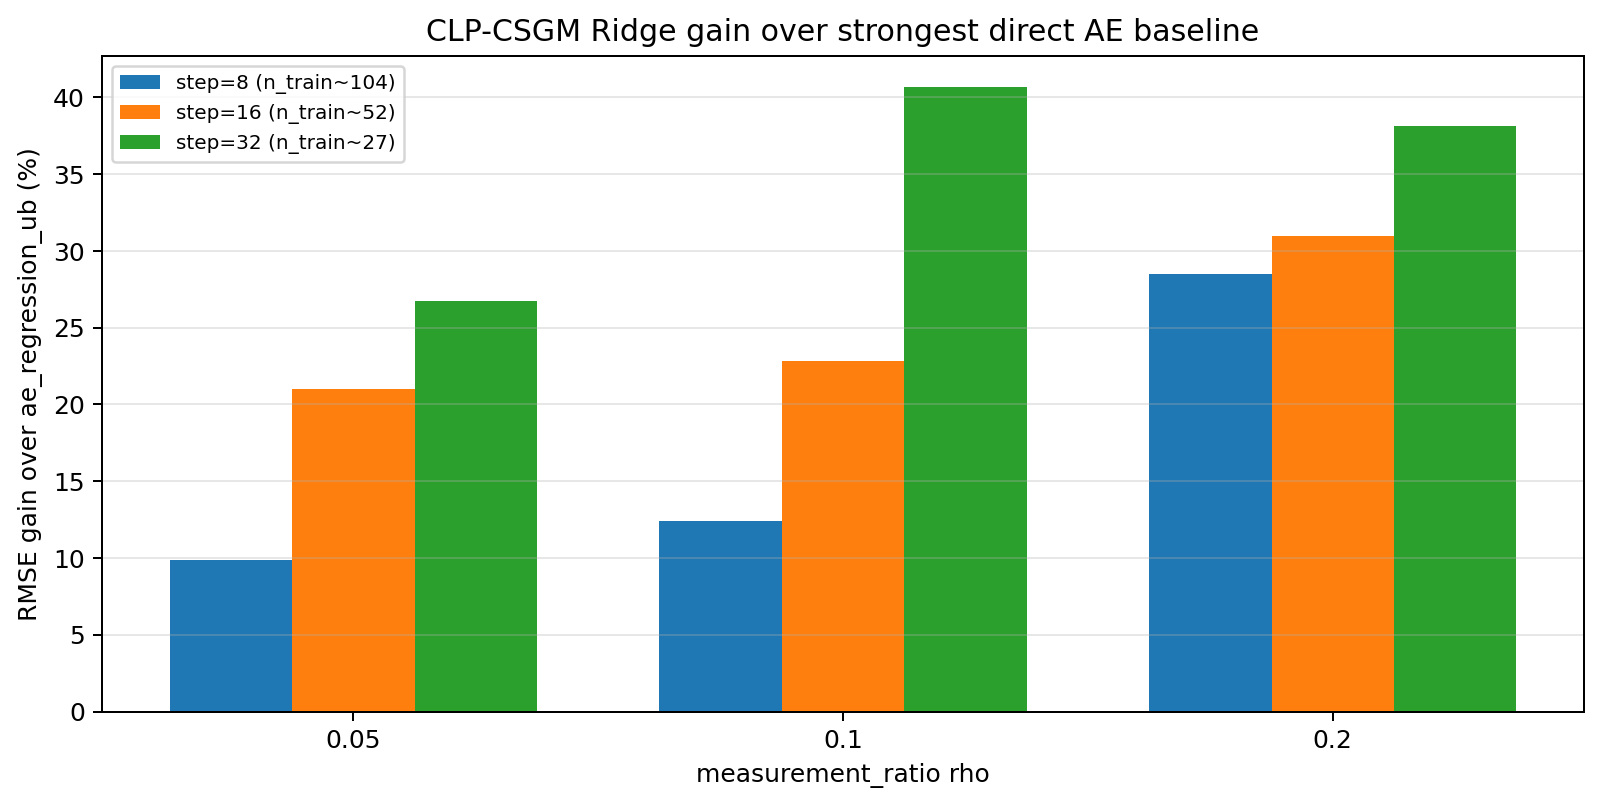
\includegraphics[width=0.82\linewidth]{figures/csgm_m2_grid/04_csgm_gain_vs_ae.png}
  \caption{RMSE gain of CLP-CSGM Ridge over the strongest previous baseline,
  \texttt{ae\_regression\_ub}. Positive values indicate CLP-CSGM improvement.}
  \label{fig:csgm_m2_gain}
\end{figure}

\begin{table}[t]
  \centering
  \caption{CLP-CSGM Ridge versus \texttt{ae\_regression\_ub} by low-data step and
  measurement ratio. Gap is relative RMSE difference of CLP-CSGM against AE; negative
  values mean CLP-CSGM is better.}
  \label{tab:csgm_m2_vs_ae}
  \small
  \begin{tabular}{@{}ccccc@{}}
    \toprule
    step & $\rho$ & CSGM RMSE & AE RMSE & gap vs AE \\
    \midrule
    $8$ & $0.05$ & $0.01541$ & $0.01709$ & $-9.84\%$ \\
    $8$ & $0.10$ & $0.01432$ & $0.01635$ & $-12.41\%$ \\
    $8$ & $0.20$ & $0.01167$ & $0.01633$ & $-28.53\%$ \\
    $16$ & $0.05$ & $0.01493$ & $0.01891$ & $-21.02\%$ \\
    $16$ & $0.10$ & $0.01391$ & $0.01803$ & $-22.81\%$ \\
    $16$ & $0.20$ & $0.01247$ & $0.01808$ & $-31.00\%$ \\
    $32$ & $0.05$ & $0.01562$ & $0.02132$ & $-26.72\%$ \\
    $32$ & $0.10$ & $0.01484$ & $0.02501$ & $-40.67\%$ \\
    $32$ & $0.20$ & $0.01259$ & $0.02035$ & $-38.15\%$ \\
    \bottomrule
  \end{tabular}
\end{table}

Across all step--rho cells, CLP-CSGM Ridge obtains mean RMSE 0.01397,
compared with 0.01905 for
\texttt{ae\_regression\_ub}, a relative gap of -26.65\%.
